\chapter{Topologies}\label{chap:topologies}
The simulations were conducted for six distinct network topologies. Each network has $2^{10}$ (1024) nodes. The behaviour of the algorithms in these different topologies is observed, since each topology has different characteristics, different performances exploiting the specials of the topologies are expected. The topologies contain the \textit{Complete graph}, \textit{Torus Grid Graph}, \textit{Ring Graph}, \textit{Star Graph}, \textit{Lollipop Graph} and \textit{Ring of Cliques}. In the following the topologies including there characteristics are presented. 

\section{Complete Graph}\label{sec:2completegraph}
The Complete graph $K_N$ as illustrated in \hyperref[fig:completegraphDemo]{figure} \ref{fig:completegraphDemo} is a graph where each pair of distinct nodes is connected by an edge. The Complete graph or also refered to as fully-connected graph has $N$ nodes and $\frac{N\times(N-1)}{2}$ edges. The Complete graph is a regular graph, where each node has a degree of $N-1$. As it contains the maximum possible number of edges for a given set of nodes (the maximum number of edges per node for undirected graphs is $N$, when self-loops are allowed), thus is a dense graph \cite{GraphTheorySchindelhaauer2021}. The diameter of a Complete graph is 1, as each node is directly connected to every other node. Since each node has same degree and connectivity, algorithms can treat all nodes uniformly. Complete graph topology is used in financial trading systems and military communications, where high reliability and low latency are critical. It ensures optimal routing paths between nodes, minimizing delays \cite{Banerjee2001}.

\begin{figure}[H]
    \centering
    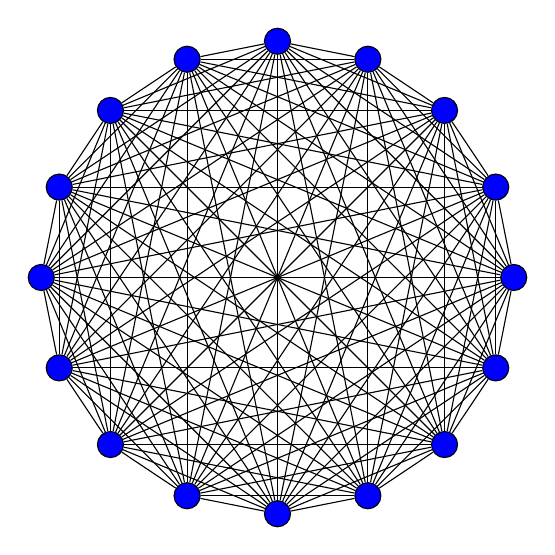
\begin{tikzpicture}
    \foreach \i in {1,...,16} {
      \node[draw, fill=blue, circle, minimum size=4pt] (v\i) at ({360/16 * (\i-1)}:3) {};
    }
    
    \foreach \i in {1,...,16} {
      \foreach \j in {1,...,16} {
        \ifnum\i<\j
          \draw (v\i) -- (v\j);
        \fi
      }
    }
    
  \end{tikzpicture}
    \caption{Complete graph: network size 16}
    \label{fig:completegraphDemo}
\end{figure}
 
\section{Torus Grid Graph}\label{sec:2torusgridgraph}
The two-dimensional Torus Grid graph or also refered to as $k \times m$-Torus graph or $T_{k,m}$ is a two-dimensional mesh with wrap around edges as depicted in \hyperref[fig:torusGraph]{figure} \ref{fig:torusGraph} \cite{Mahlmann2010}. $k$ denotes the height and $m$ denotes the width of the grid. The Torus Grid graph has $2\times k \times m$  edges (if $k, m$ > 2) and $k \times m$ nodes and is a regular graph, where each node has a degree of 4. The diameter of a Torus Grid graph is $\frac{min(k,m)}{2}$. Tori are scalable, as the number of connections per node is constant, regardless of the graph size. In the previous research "Comparative Analysis of Load Balancing Algorithms in General Graphs" \cite{Bayazitoglu}, the simulation results showed to not vary over different network sizes. Torus topology is prevalent in supercomputers like IBM Blue Gene and Cray systems for high-performance computing. It is also implemented in Network-on-Chip (NoC) designs for its ability to handle data distribution with low latency and high fault tolerance. Torus topology is commonly found in Fiber Distributed Data Interface (FDDI) and Synchronous Optical Networking (SONET) for local and metropolitan area networks. \cite{Banerjee2001}.

\begin{figure}[H]
    \centering
    \scalebox{1.5}{\tikzset{
    block/.style={draw, fill=blue, circle, minimum size=3pt},
    arrow/.style={->},
    line/.style={-}
}

\begin{tikzpicture}[>=stealth',node distance=0.5cm]
    % Creating rows of blocks
    {[start chain]
        \node[on chain] (s0) {};
        \node[on chain] (s1) {};
        \node[on chain] (s2) {};
        \node[on chain] (s3) {};
        \node[on chain] (s4) {};
    }
    {[start chain]
        \node[block,on chain, below = 0.15 cm of s0] (A0) {};
        \node[block,on chain, join =by {line}] (A1) {};
        \node[block,on chain, join =by {line}] (A2) {};
        \node[block,on chain, join =by {line}] (A3) {};
    }
    {[start chain]
        \node[block,on chain, below = of A0] (B0) {};
        \node[block,on chain, join =by {line}] (B1) {};
        \node[block,on chain, join =by {line}] (B2) {};
        \node[block,on chain, join =by {line}] (B3) {};
    }
    {[start chain]
        \node[block,on chain, below = of B0] (C0) {};
        \node[block,on chain, join =by {line}] (C1) {};
        \node[block,on chain, join =by {line}] (C2) {};
        \node[block,on chain, join =by {line}] (C3) {};
    }
    {[start chain]
        \node[block,on chain, below = of C0] (D0) {};
        \node[block,on chain, join =by {line}] (D1) {};
        \node[block,on chain, join =by {line}] (D2) {};
        \node[block,on chain, join =by {line}] (D3) {};
    }

    % Drawing vertical lines
    \draw (A0) -- (B0) -- (C0) -- (D0); % -- (E0);
    \draw (A1) -- (B1) -- (C1) -- (D1); % -- (E1);
    \draw (A2) -- (B2) -- (C2) -- (D2); % -- (E2);
    \draw (A3) -- (B3) -- (C3) -- (D3); % -- (E3);
    % Drawing loop backs horizontal
    \draw (A0.west) -- ($(A0.west) - (0.15, 0)$);
    \draw ($(A0.west) - (0.15, 0)$) -- ($(A0.west) - (0.15, 0)+(0,0.5)$);
    \draw ($(A0.west) - (0.15, 0)+(0,0.5)$) -- ($(A0.west) +(3.1,0.5)$);
    \draw ($(A0.west) +(3.1,0.5)$) |- (A3.east);
    % \draw (A0.north) |- (s2.north east) -| (A4.north);
    % B row
    \draw (B0.west) -- ($(B0.west) - (0.15, 0)$);
    \draw ($(B0.west) - (0.15, 0)$) -- ($(B0.west) - (0.15, 0)+(0,0.5)$);
    \draw ($(B0.west) - (0.15, 0)+(0,0.5)$) -- ($(B0.west) +(3.1,0.5)$);
    \draw ($(B0.west) +(3.1,0.5)$) |- (B3.east);
    % C row
    \draw (C0.west) -- ($(C0.west) - (0.15, 0)$);
    \draw ($(C0.west) - (0.15, 0)$) -- ($(C0.west) - (0.15, 0)+(0,0.5)$);
    \draw ($(C0.west) - (0.15, 0)+(0,0.5)$) -- ($(C0.west) +(3.1,0.5)$);
    \draw ($(C0.west) +(3.1,0.5)$) |- (C3.east);
    % D row
    \draw (D0.west) -- ($(D0.west) - (0.15, 0)$);
    \draw ($(D0.west) - (0.15, 0)$) -- ($(D0.west) - (0.15, 0)+(0,0.5)$);
    \draw ($(D0.west) - (0.15, 0)+(0,0.5)$) -- ($(D0.west) +(3.1,0.5)$);
    \draw ($(D0.west) +(3.1,0.5)$) |- (D3.east);

    % Vertical Loopbacks

    % 0 column
    \draw (A0.north) -- ($(A0.north) + (0.0, 0.15)$);
    \draw ($(A0.north) + (0, 0.15)$) -- ($(A0.north) + (0, 0.15)+(-0.5,0)$);
    \draw ($(A0.north) + (0, 0.15)+(-0.5,0)$) -- ($(D0.north) +(-0.5,-0.65)$);
    \draw ($(D0.north) +(-0.5,-0.65)$) -| (D0.south);
    % 1 column
    \draw (A1.north) -- ($(A1.north) + (0.0, 0.15)$);
    \draw ($(A1.north) + (0, 0.15)$) -- ($(A1.north) + (0, 0.15)+(-0.5,0)$);
    \draw ($(A1.north) + (0, 0.15)+(-0.5,0)$) -- ($(D1.north) +(-0.5,-0.65)$);
    \draw ($(D1.north) +(-0.5,-0.65)$) -| (D1.south);
    % 2 column
    \draw (A2.north) -- ($(A2.north) + (0.0, 0.15)$);
    \draw ($(A2.north) + (0, 0.15)$) -- ($(A2.north) + (0, 0.15)+(-0.5,0)$);
    \draw ($(A2.north) + (0, 0.15)+(-0.5,0)$) -- ($(D2.north) +(-0.5,-0.65)$);
    \draw ($(D2.north) +(-0.5,-0.65)$) -| (D2.south);

    % 3 column
    \draw (A3.north) -- ($(A3.north) + (0.0, 0.15)$);
    \draw ($(A3.north) + (0, 0.15)$) -- ($(A3.north) + (0, 0.15)+(-0.5,0)$);
    \draw ($(A3.north) + (0, 0.15)+(-0.5,0)$) -- ($(D3.north) +(-0.5,-0.65)$);
    \draw ($(D3.north) +(-0.5,-0.65)$) -| (D3.south);
    
    \end{tikzpicture}}
    \caption{Torus grid graph: network size 16}
    \label{fig:torusGraph}
\end{figure}

\section{Ring Graph}\label{sec:2ringgraph}
The Ring graph $R_N$ is a regular graph, where each node has a degree of two, forming a cycle. The Ring graph can be constructed by building a Path graph which is closed, meaning that the first and the last nodes of the Path graph are connected by an edge as depicted in \hyperref[fig:ring]{figure } \ref{fig:ring}. The graph consists of $N$ nodes and $N$ edges. The diameter of a ring is $\lfloor{\frac{N}{2}}\rfloor$. The uniform structure ensures no single node has an advantage, simplifying algorithm design and guaranteeing fairness in load balancing.  Most of the Ring structures use a token-based communication model. The node that holds the taken may transmit data. Most of current high speed LANs have a Ring topology \cite{Vidomenko1997}. The advantage of an Ring graph is that when faults occur the troubleshooting is relatively easy. However, a single outage of a node may disrupt the whole network activity.

\begin{figure}[H]
    \centering
    \scalebox{0.8}{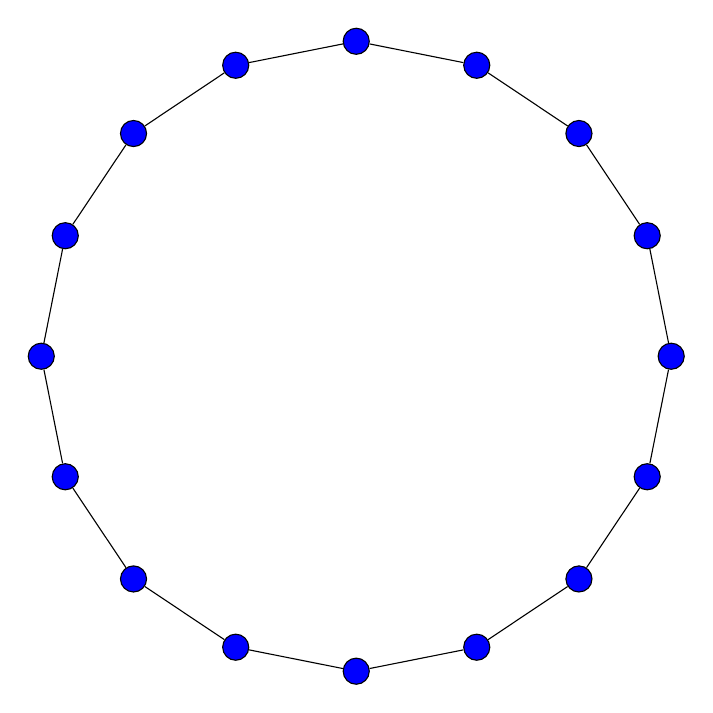
\begin{tikzpicture}
  \def\nodes{16}
  \def\radius{4}
  \foreach \i in {1,...,\nodes} {
      \node[draw, fill=blue, circle, minimum size=6pt] (v\i) 
      at ({\i*360/\nodes}: \radius) {};
  }

  \foreach \i in {1,...,\nodes} {
      \pgfmathtruncatemacro{\j}{mod(\i, \nodes) + 1}
      \draw (v\i) -- (v\j);
  }
\end{tikzpicture}}
    \caption{Ring graph: network size 16}
    \label{fig:ring}
\end{figure}

\section{Star Graph}\label{sec:2stargraph}
A Star graph $S_N$ as depicted in \hyperref[fig:stargraphDemo]{figure} \ref{fig:stargraphDemo} is a bipartite graph \cite{west2001introduction}, structured like a tree graph with one internal node and k-leaves. A Star graph with $N$ nodes has $N-1$ edges. In this structure, every leaf node has a degree of 1, meaning it is connected only to the internal node. The central node has a degree of $N-1$. The diameter of a star graph is 2 (path from one leave through internal node to another leave). Regarding load balancing the internal node acts as a point of redistribution. This topology is particularly suitable for master-slave or client-server models where the central node delegates tasks and collects results. However, the central node may become overloaded in high-load scenarios, requiring careful design to prevent bottlenecks. A common usage for the Star topology is a LAN (Local Area Network) in home networks, where all devices are connected to a hub or the router \cite{Jayeola2023}. The challenge when dealing with Star graphs is that the failure of the central node (hub or router) shuts down the whole network. The advantage of such a setting is that adding new devices is simple and failures of leaf nodes do not affect the whole network.

\begin{figure}[H]
    \centering
    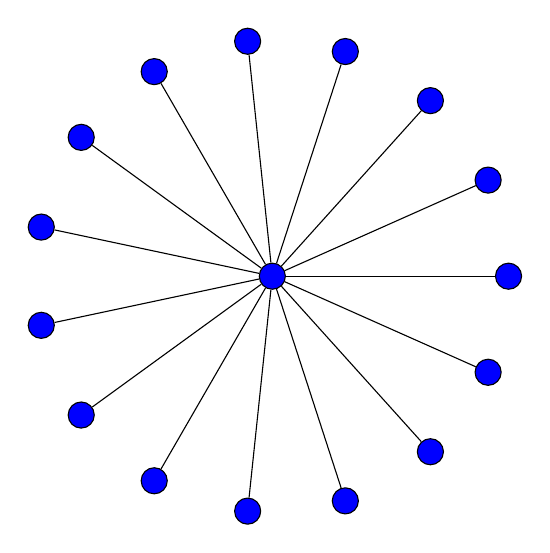
\begin{tikzpicture}
    \node[draw, fill=blue, circle, minimum size=6pt] (center) at (0, 0) {};
    \foreach \i in {1,...,15} {
            \node[draw, fill=blue, circle] (n\i) at ({360/15 * (\i-1)}:3) {};
            \draw (center) -- (n\i);
        }
\end{tikzpicture}
    \caption{Star graph: network size 16}
    \label{fig:stargraphDemo}
\end{figure}


\section{Lollipop Graph}\label{sec:2lollipopgraph}
A $(k, m)$-Lollipop graph $L_{k,m}$ is a graph that consists of a Complete graph and a Path graph as depicted in \hyperref[fig:lollipopgraphDemo]{figure} \ref{fig:lollipopgraphDemo}. The Complete graph and the Path graph are connected by a bridge node, thus a single edge. The $(k, m)$-Lollipop graph is composed of a Complete graph with $k$ nodes and a path size of $m$ nodes. A Lollipop graph has $N$ nodes, where $N = k+m$ and $(\frac{k*(k-1)}{2})+m$ edges \cite{JonassonLollipopGraphs2000}.

\begin{figure}[H]
    \centering
    \scalebox{1}{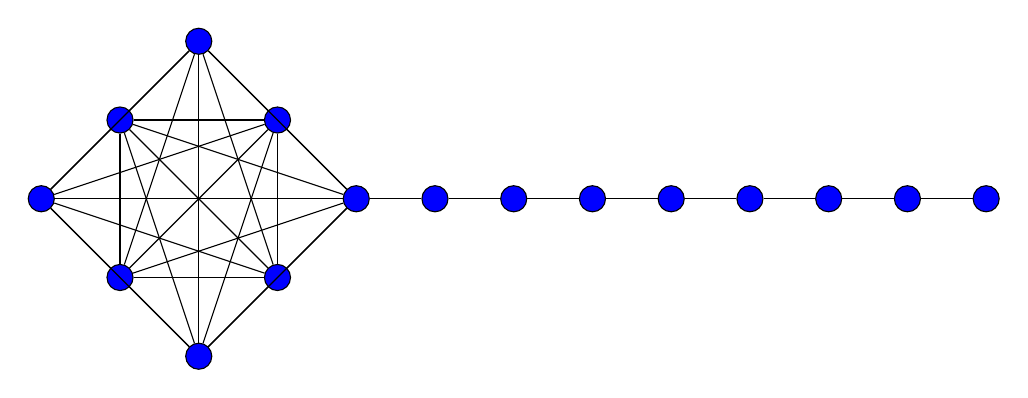
\begin{tikzpicture}
    % Define the 8 vertices in a flat line
    \foreach \i in {1,...,9} {
      \node[draw, fill=blue, circle, minimum size=6pt] (v\i) at (\i, 0) {};
    }
    
    % Draw edges to connect each vertex to the next
    \foreach \i in {1,...,8} {
      \pgfmathtruncatemacro{\j}{\i+1}
      \draw (v\i) -- (v\j);
    }

    % Define additional vertices for the complete graph on v1, centered around v1
    \node[draw, fill=blue, circle, minimum size=6pt] (c1) at (0,1) {};
    \node[draw, fill=blue, circle, minimum size=6pt] (c2) at (0,-1) {};
    \node[draw, fill=blue, circle, minimum size=6pt] (c3) at (-1,2) {};
    \node[draw, fill=blue, circle, minimum size=6pt] (c4) at (-1,-2) {};
    \node[draw, fill=blue, circle, minimum size=6pt] (c5) at (-2,-1) {};
    \node[draw, fill=blue, circle, minimum size=6pt] (c6) at (-2,1) {};
    \node[draw, fill=blue, circle, minimum size=6pt] (c7) at (-3, 0) {};
    
    % Connect the complete graph nodes to v1
    \foreach \k in {1,2,3,4,5,6,7} {
      \draw (v1) -- (c\k);
    }

    % Draw edges between the new nodes to form a complete graph
    \foreach \a in {1,2,3,4,5,6,7} {
      \foreach \b in {\a,...,7} {
        \ifnum\a=\b\else
        \draw (c\a) -- (c\b);
        \fi
      }
    }

  \end{tikzpicture}}
    \caption{Lollipop graph: network size 16}
    \label{fig:lollipopgraphDemo}
\end{figure}

\section{Ring of Cliques}\label{sec:2ringofcliquegraph}
The ($k \times m$)-Ring of Cliques $ROC_{k,m}$, consists of $k$ cliques, each containing $m$ nodes. The cliques are connected to form a ring structure. To create the ring, one edge from each clique is removed, and the endpoints of these removed edges are connected to form a regular graph \cite{Mahlmann2010}. A $k \times m$ ring of cliques has $\left( k\times \left(\frac{m\times (m - 1)}{2}-1 \right) \right)+k$ edges. The connectivity of the graph increases with larger clique sizes and decreases with smaller clique sizes.

\begin{figure}[H]
    \centering
    \scalebox{1}{\newcommand\single[2]{
\foreach \x in {1,...,#2}{
\pgfmathsetmacro{\ang}{360/#2}
    \pgfmathparse{(\x-1)*\ang}
    \node[draw, fill=blue, circle, minimum size=6pt] (#1-\x) at (\pgfmathresult:10cm) {};
  }
  \foreach \x [count=\xi from 1] in {2,4}{
            \foreach \y in {2,4}{
                    \path (#1-\xi) edge[-] (#1-\y);
                    \path (#1-3) edge[-] (#1-\y);
                }
        }
}

\begin{tikzpicture}
    \begin{scope}[local bounding box=scope1]
    \end{scope}

    \foreach \s[count=\si from 0] in {0,90,...,360}{
        \begin{scope}[shift={($(scope1) +(\s:2)$)}, scale=0.1, rotate=\s+90]
            \single{\si}{4};
        \end{scope}
    }

    \foreach \i/\j in {1/2, 2/3, 3/4, 4/1}{
        \ifnum\i=1
            \draw[thick] (\i-1) to[out=180, in=90] (\j-3);
        \else\ifnum\i=2
            \draw[thick] (\i-1) to[out=-90, in=180] (\j-3);
        \else\ifnum\i=3
            \draw[thick] (\i-1) to[out=0, in=-90] (\j-3);
        \else
            \draw[thick] (\i-1) to[out=90, in=0] (\j-3);
        \fi\fi\fi
    }
\end{tikzpicture}

}
    \caption{Ring of Cliques: network size 16}
    \label{fig:ringofcliquesDemo}
\end{figure}

\section{Expected Outcome}\label{sec:expectedoutcome}
Many load balancing algorithms perform well on 2D Tori due to the focus on local redistribution, thanks to the wrap around edges eliminiating boundary effects, ensuring balanced redistribution across entire grid.

For the Ring graphs, where unlike complete or torus graphs, the sequential nature of data transfer makes it slower for loads to propagate across the entire Ring. Load movement in the Ring graph is sequential, making it slower and less flexible than the Complete graph.

Star: For the Push-Pull mechanism the star graph is an advantage, since each push action contains a pull action. All leaves request data from the internal node, so the internal node acts here as an point of redistribution. However for the Deal-Agreement-Based protocol some mechanisms like "if condition" act as a contraproductive way of load balancing.

Lollipop: Algorithms must account for the highly connected complete graph (dense communication) and the linear path graph (sequential communication), which introduces a mixed topology challenge. The node linking the complete graph and the path graph often becomes a bottleneck since it bridges two vastly different connectivity regions. In the complete graph, load balancing is efficient due to the high connectivity, enabling rapid redistribution among nodes. Load movement in the path graph is sequential, making it slower and less flexible than the complete graph. Interesting because dense head and sparse tail.  For example, diffusion-based approaches work well in the head but may require additional iterations in the tail. We saw that in "Comparative Analysis of Load Balancing algorithms in General Graphs" \cite{Bayazitoglu}, once we changed the path size in relation to same complete graph, the DAB was faster in reducing error for the first 50 rounds. \todo{Do the simulations over again with different path and complete graph size and compare.}

Ring of cliques: Within each clique, balancing is fast due to the dense connectivity. Load redistributes efficiently among the clique's nodes. Balancing between cliques depends on the single shared node linking each pair of cliques. This structure ensures sequential redistribution across the ring. The shared nodes act as gateways, controlling the flow of load between cliques. Overloading these nodes can cause bottlenecks.